\section{Expanding the Task Space: Grasping Tasks}\label{sec:grasping-tasks}
A grasping task will likely suffer from a lack of viewing poses I first designed a simple version (Figure \ref{fig:grasp}) which the agent learns to reach then grasp the cubic target. Main differences between this and the reaching task is that the target here is tangible, so on top of being rendered it is also set to be \emph{collidable}. Another major addition is the usage of the \emph{extension string} as seen in \ref{subfig:simple-zoom-actions}, this instructs the demonstration engine to insert certain moves within the calculated trajectory. In this case \verb|open_gipper()| ensures the gripper is open; then a later waypoint will instruct it to close. 

Final difference to mention is the cubic target. This was a quality of life choice, the spherical object was simple to attempt to grab. During initial experimentation, I realised that the agent would try to grab the top bit of the sphere, get no grip but the simulator would report a successful grab. Realising this was likely due to the geometry of the target, I changed it to use a cube shape, which solved the issues.\todo[color=purple]{}. The more complicated counterpart, shown in Figure \ref{fig:grasp-front}, is a scenario where the cube needs to be picked up then moved to the target location (designated in green). I suspect this task will be challenging. Once the cube is picked up, its field of vision will be significantly occluded by the target\todo[color=red]{add a picture with the cube grasped and the wrist camera view seen at that point}, and the agent will likely not see the green landing. Therefore, multiple views and remembering the environment from the initial pose might play a big role.

\begin{figure}[htpb] % htpb allows all placement
  \centering
  \begin{subfigure}{0.2\linewidth}
    \centering
    \includegraphics[width=0.7\linewidth]{../fyp/assets/task-pics/grasp/simple-front.png}
    \caption{Front}\label{subfig:simple-front}
  \end{subfigure}
  \begin{subfigure}{0.3\linewidth}
    \centering
    \includegraphics[width=0.9\linewidth]{../fyp/assets/task-pics/grasp/simple-front-zoom-gripper_actions.png}
    \caption{Zoomed, with gripper action}\label{subfig:simple-zoom-actions}
  \end{subfigure}
  \begin{subfigure}{0.2\linewidth}
    \centering
    \includegraphics[width=0.7\linewidth]{../fyp/assets/task-pics/grasp/move-front.png} 
    \caption{Front}\label{subfig:grasp-move-front}
  \end{subfigure}
  \begin{subfigure}{0.2\linewidth}
    \centering
    \includegraphics[width=0.7\linewidth]{../fyp/assets/task-pics/grasp/move-top.png}
    \caption{Top}\label{subfig:grasp-move-top}
  \end{subfigure}
  \caption{Simple Grasping Task}\label{fig:grasp}
\end{figure}

\subsection{Creating an Appropriate Policy}
The previous policy would regress the entire 6DoF along with the final \emph{float} that controls the gripper. This was evident earlier when observing the reaching task I realised the gripper would sometimes `clap', meaning it would open and close quickly for every other action, which is odd, but was not a deal breaker before.

This is not sufficient, there weren't many frames the gripper is signaled to be closed, as the gripping happens at the end of the task; means that there is an inherent imbalance in our dataset. If we were to treat \textbf{CLOSED} and \textbf{OPEN} as binary labels; which they are as RLBench takes a \emph{float} $\in \left[0, 1\right]$ and thresholds at $ > 0.9$ to check if it should be open. Therefore, regressing the entire action skews it to staying open.

To adjust for this I first tried to do binary classification with weighting the samples to counteract this, which was not fruitful just due to the overall dataset size being small as well. There are as much data as there is episodes in a demo, which is usually not much more than $50$. So, going back to regression, I decided to add Binary Cross Entropy (BCE) Loss; using \verb|BCEWithLogitsLoss| from Pytorch \cite{pytorch}. Along with a gripper prediction head just to predict the gripper action from the extracted camera features, then add this as a part of the overall loss with a weighting, giving us:

\[
  loss = loss_{mse} \left(action_{v}, ~\widehat{action_v}\right) 
  + 
  \lambda_{gripper} loss_{bce}\left( action_{g}, ~\widehat{action_g}\right)
\]

where $v$ and $g$ means respectively the $7$-dim joint velocity vector and the $1$-dim float vector which is \( \in \{ 0.0, 1.0 \}\) Making the gripper separately tunable. This makes inherent sense as the movement decisions should never affect the gripper. The information flow is camera to movement and gripper action separately.

\subsection{Observations}\todo{maybe remove or move down}

\begin{figure}[htpb] % htpb allows all placement
  \centering
  \begin{subfigure}{0.45\linewidth}
    \centering
    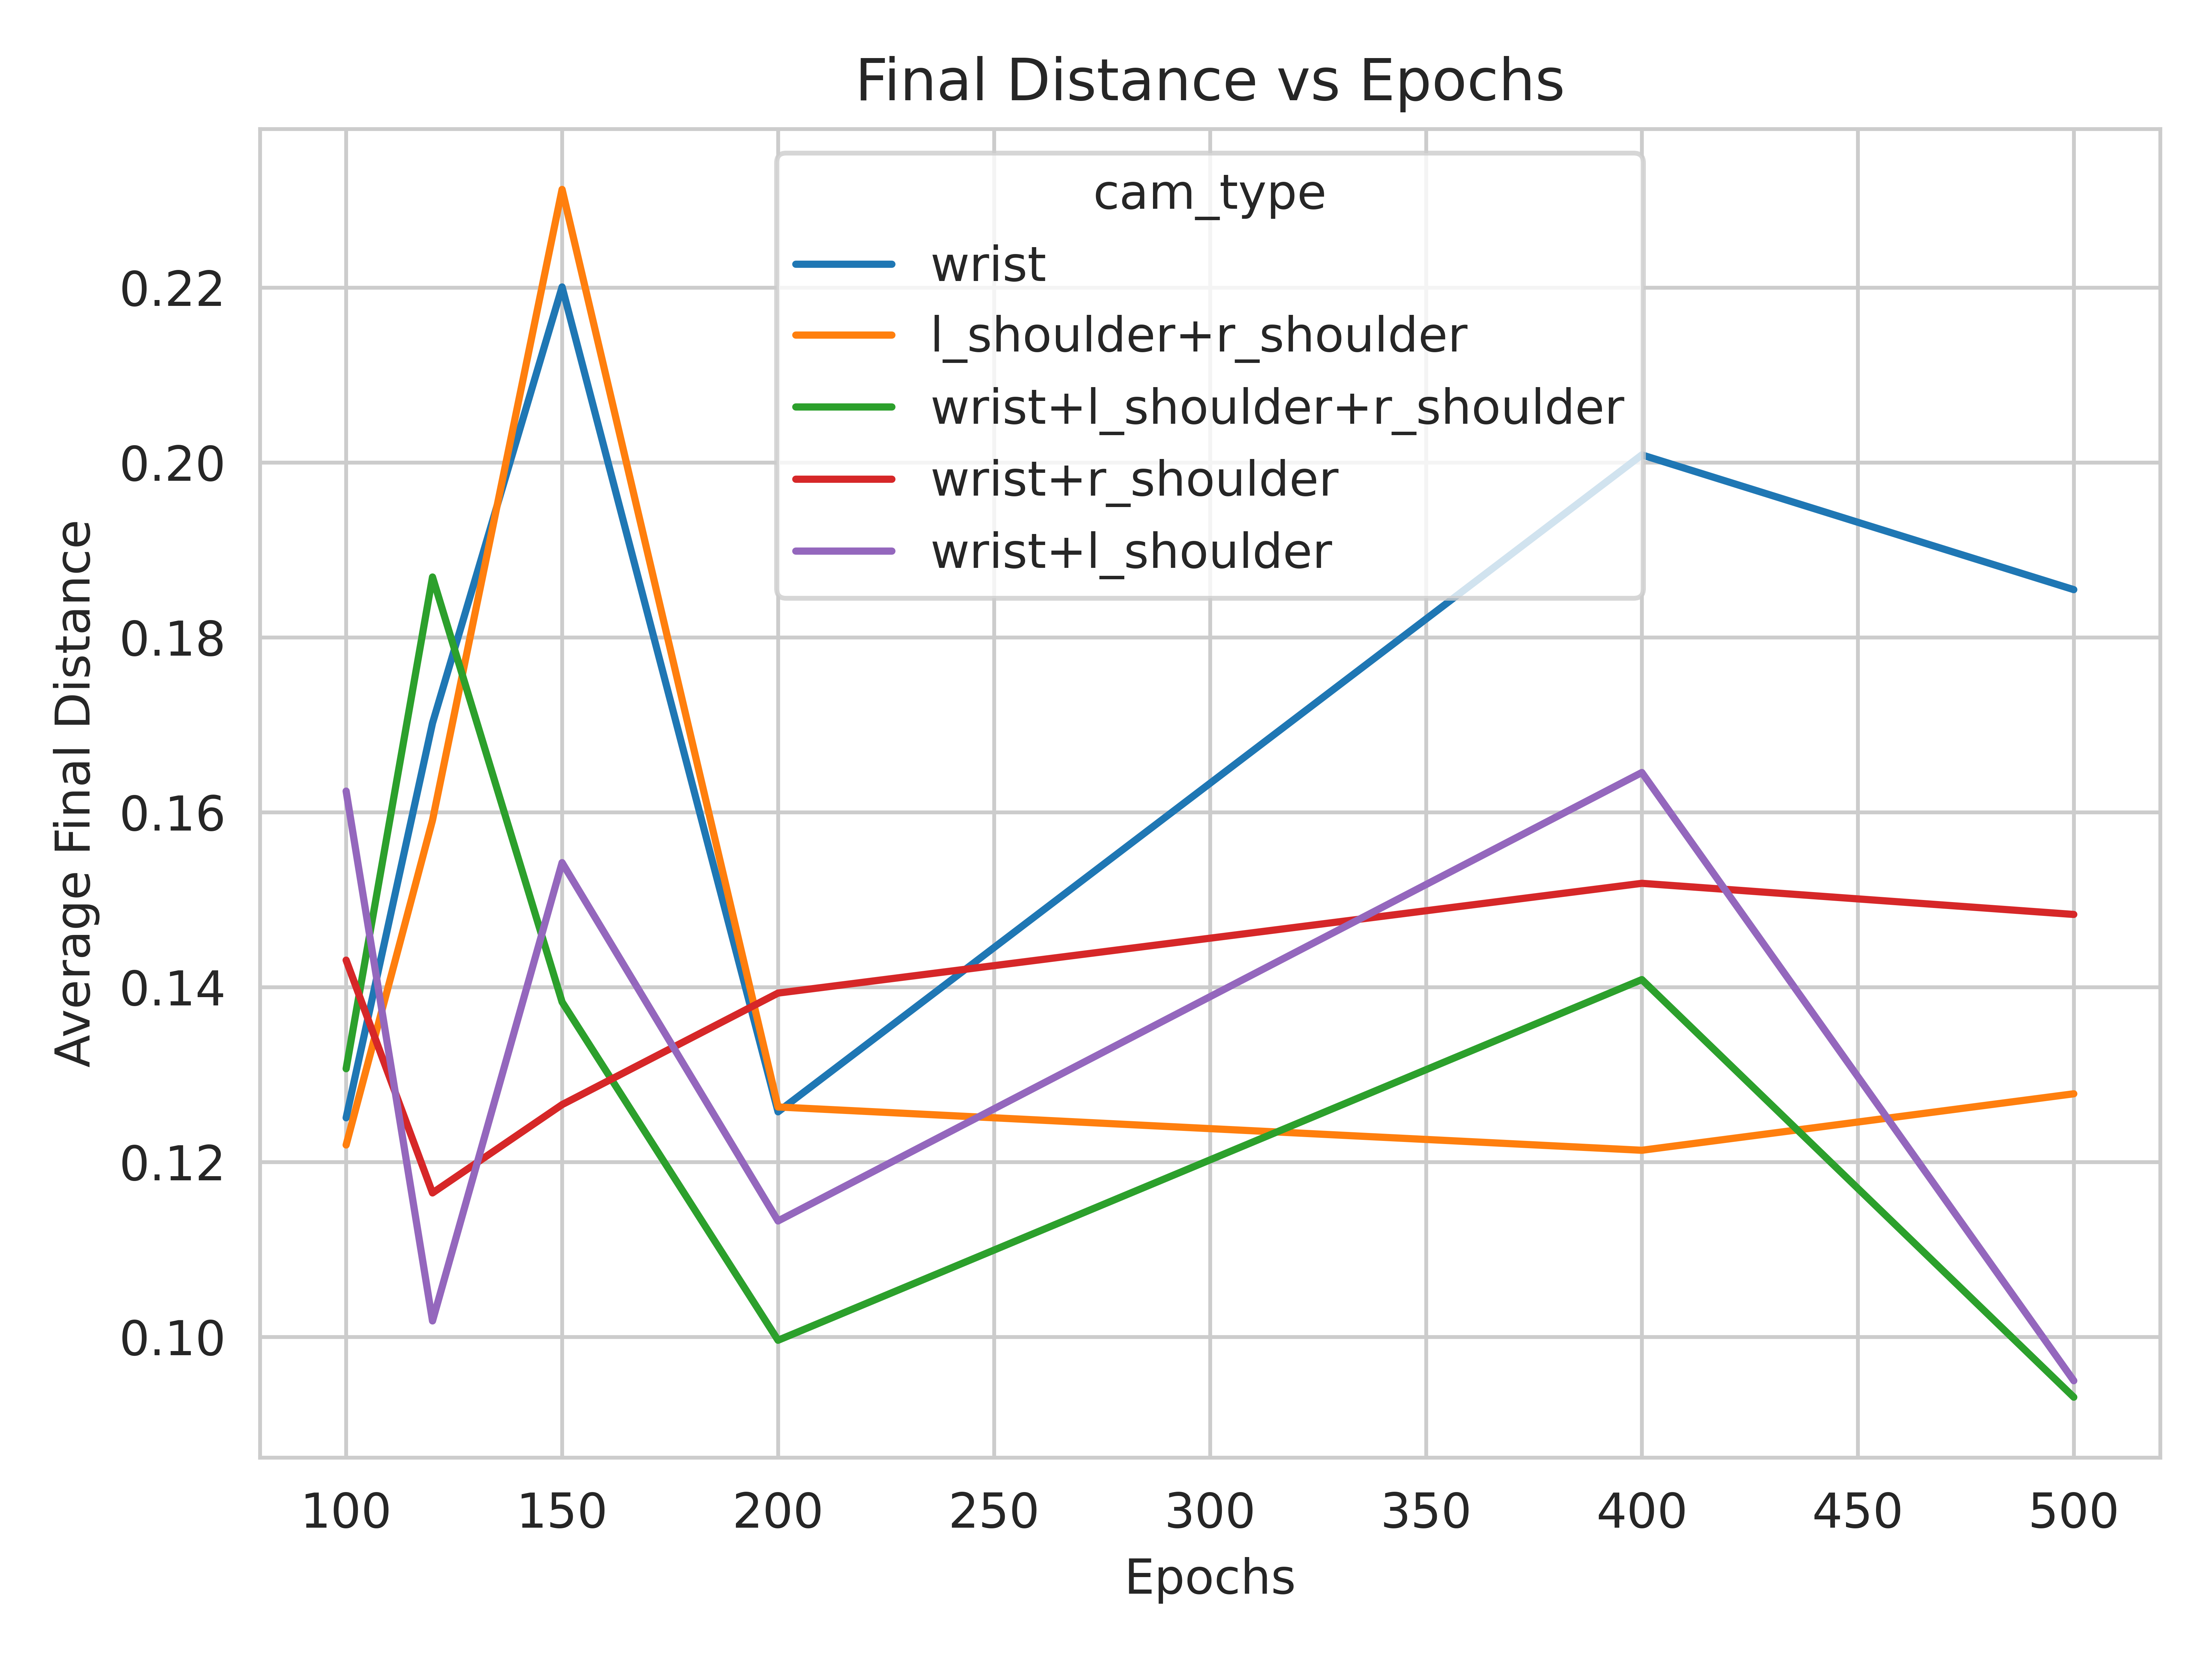
\includegraphics[width=0.7\linewidth]{assets/cam-comb/grasp-simple/tuning-normal-old-policy-dist.png}
    \caption{Average Final Distance vs Training Epochs}\label{subfig:grasp-tuning-dist}
  \end{subfigure}
  % \hfill
  \begin{subfigure}{0.45\linewidth}
    \centering
    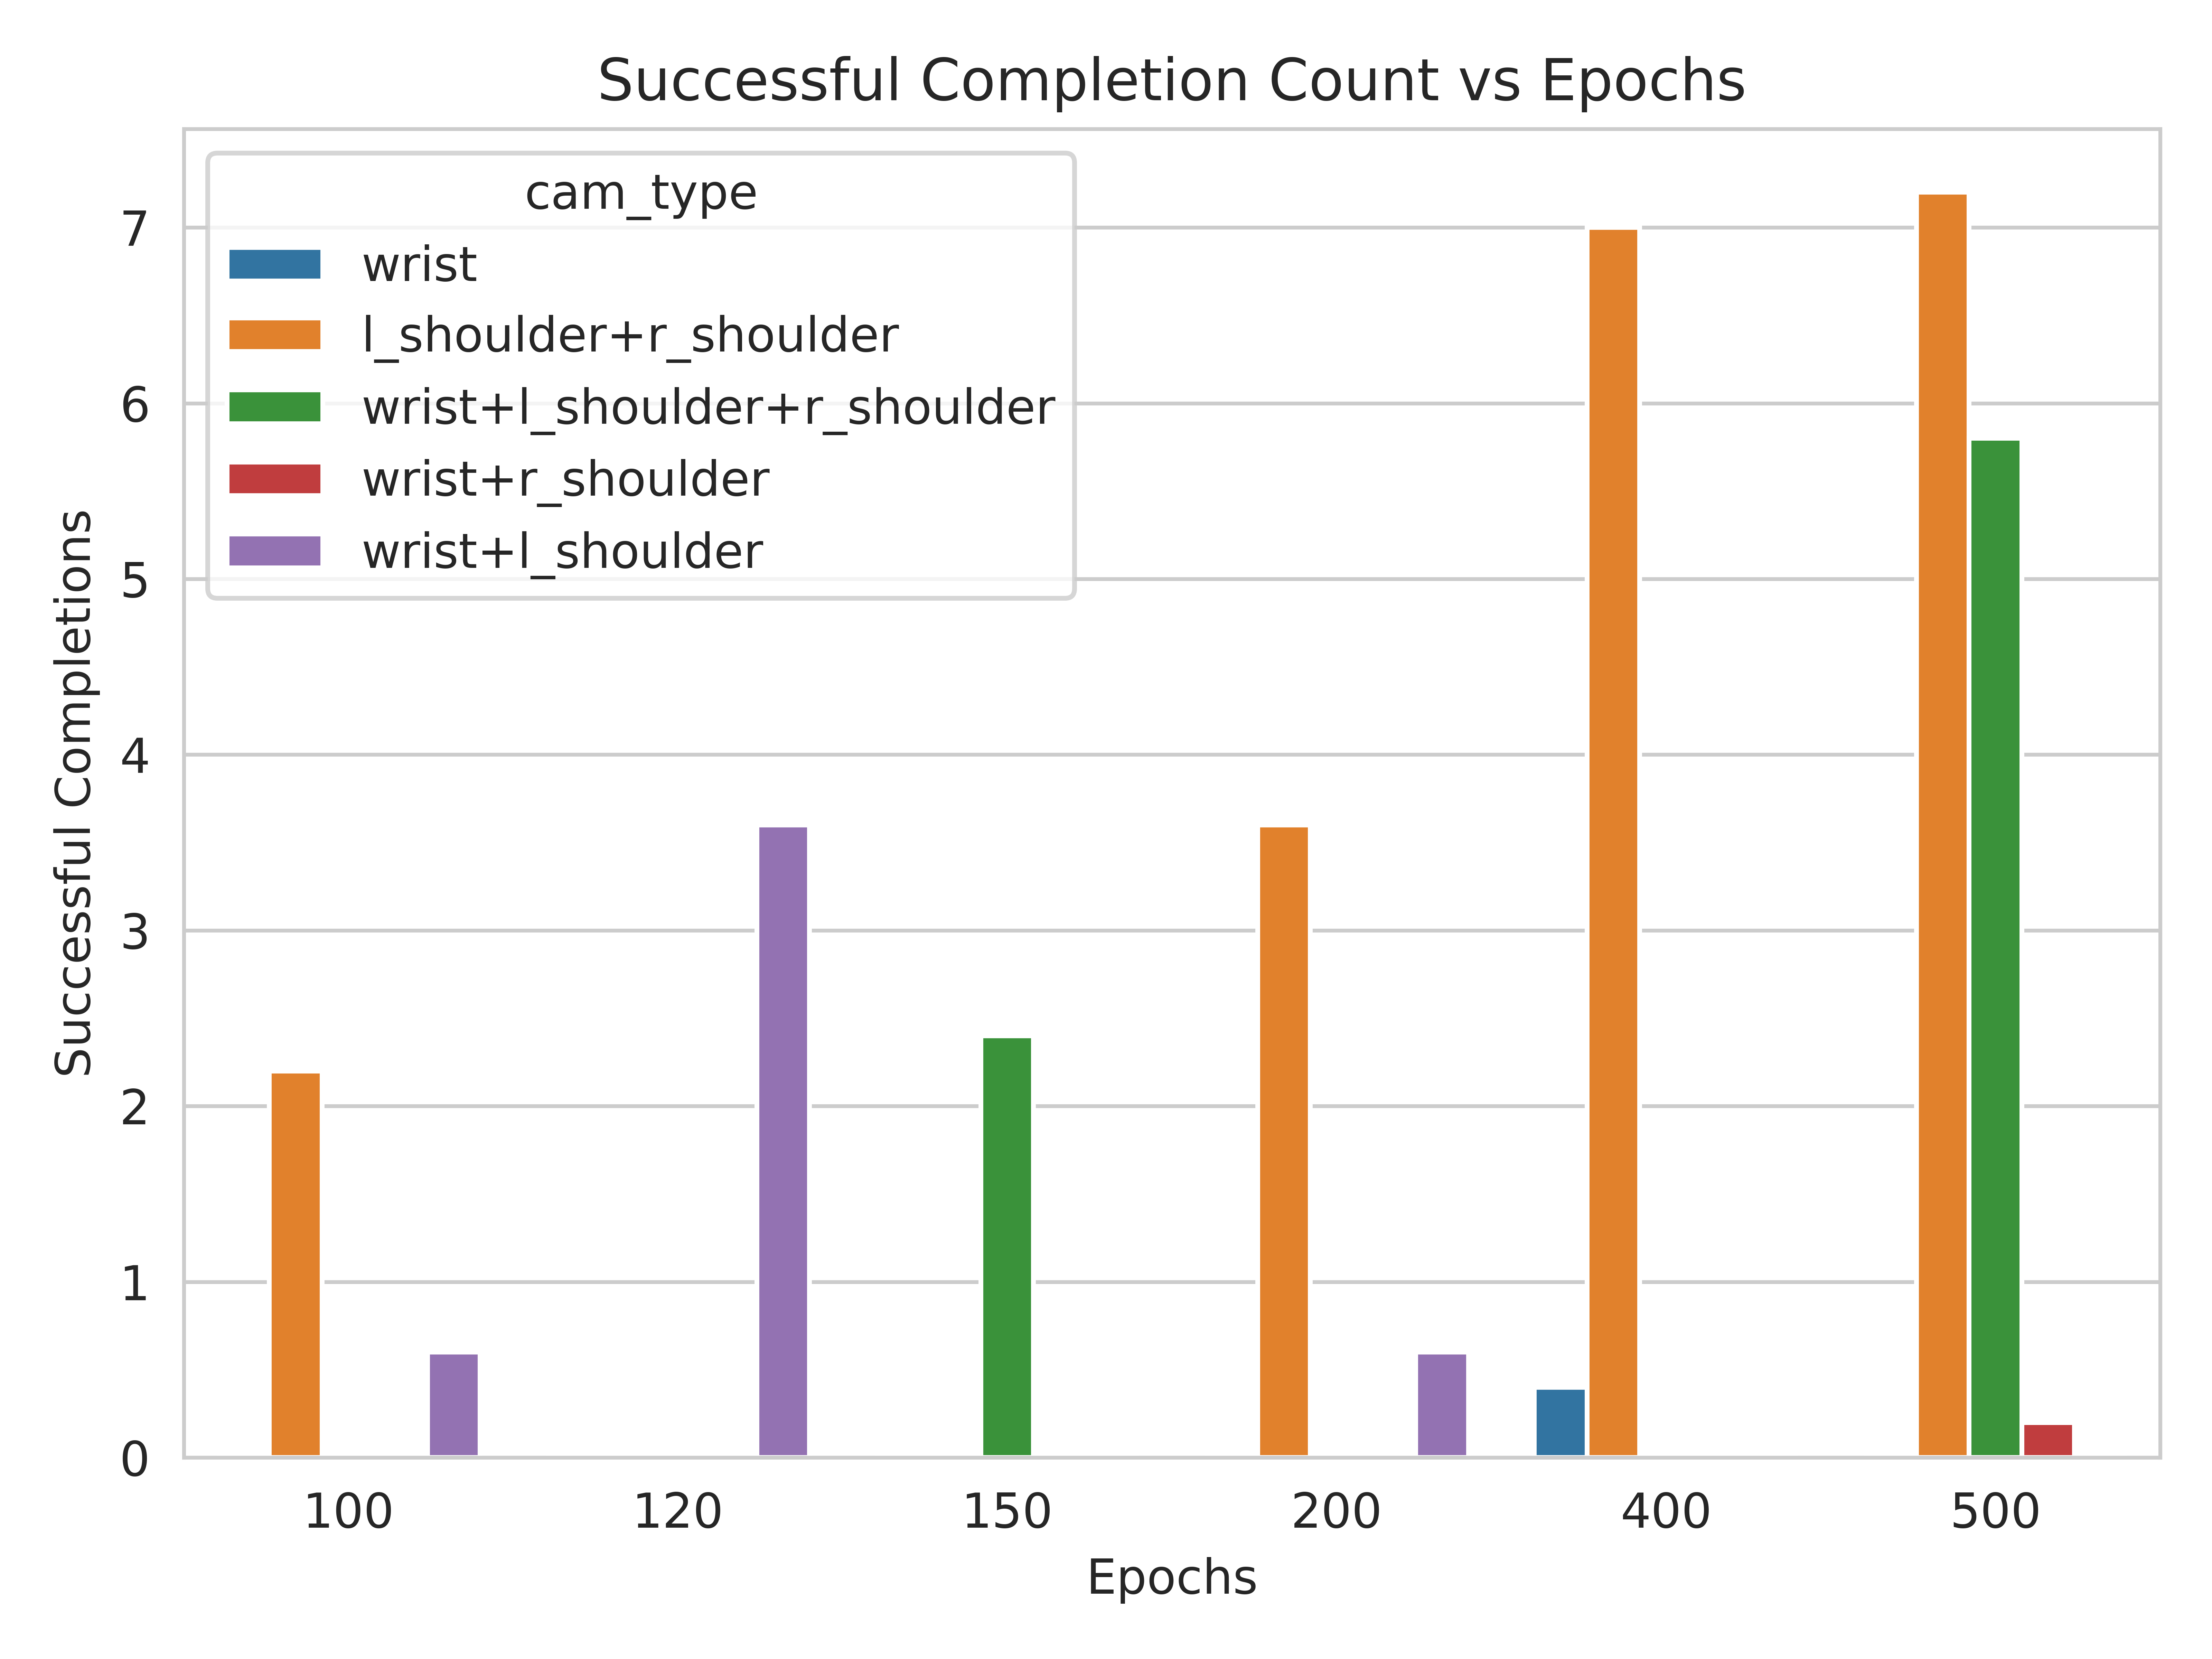
\includegraphics[width=0.7\linewidth]{assets/cam-comb/grasp-simple/tuning-normal-old-policy-success.png}
    \caption{Successful Completions vs Training Epochs}\label{subfig:grasp-tuning-dist-success}
  \end{subfigure}
  \caption{Simple Grasp Tuning: Each combination of parameters are repeated 10 times over testing data and results are averaged}\label{fig:grasp-tuning-epochs}
\end{figure}

\subsection{The Grasp}
The biggest challenge was to tune the success rate of the tests. The agent was good at reaching towards the target, as evident from the fairly low minimum and final distances \ref{subfig:grasp-tuning-dist}. An observation from these task is that learning the reaching movement does not take very many epochs as seen before in \ref{sec:reach-no-obs} However, unlike the reaching task, the success of this task is dependent on getting a correct grasp which it is not very good at.

\subsubsection{Augmenting the Loss}
My initial response was to tweak and weight the grasping loss component, $\lambda_{gripper}$. However, increasing it too much meant the movement wasn't being learnt well -neither the grasping as, open data is more abundant. While keeping it too low, means no grasping is learnt. After experimenting, I figured out that \(\left[0.9, 1.2\right]\) was the optimal range \ref{fig:grasp-tuning-lambda-g}, where the loss terms didn't dominate each other. $1$ and $1.2$ are the best performers

\begin{figure}[htpb] % htpb allows all placement
  \centering
  \begin{subfigure}{0.45\linewidth}
    \centering
    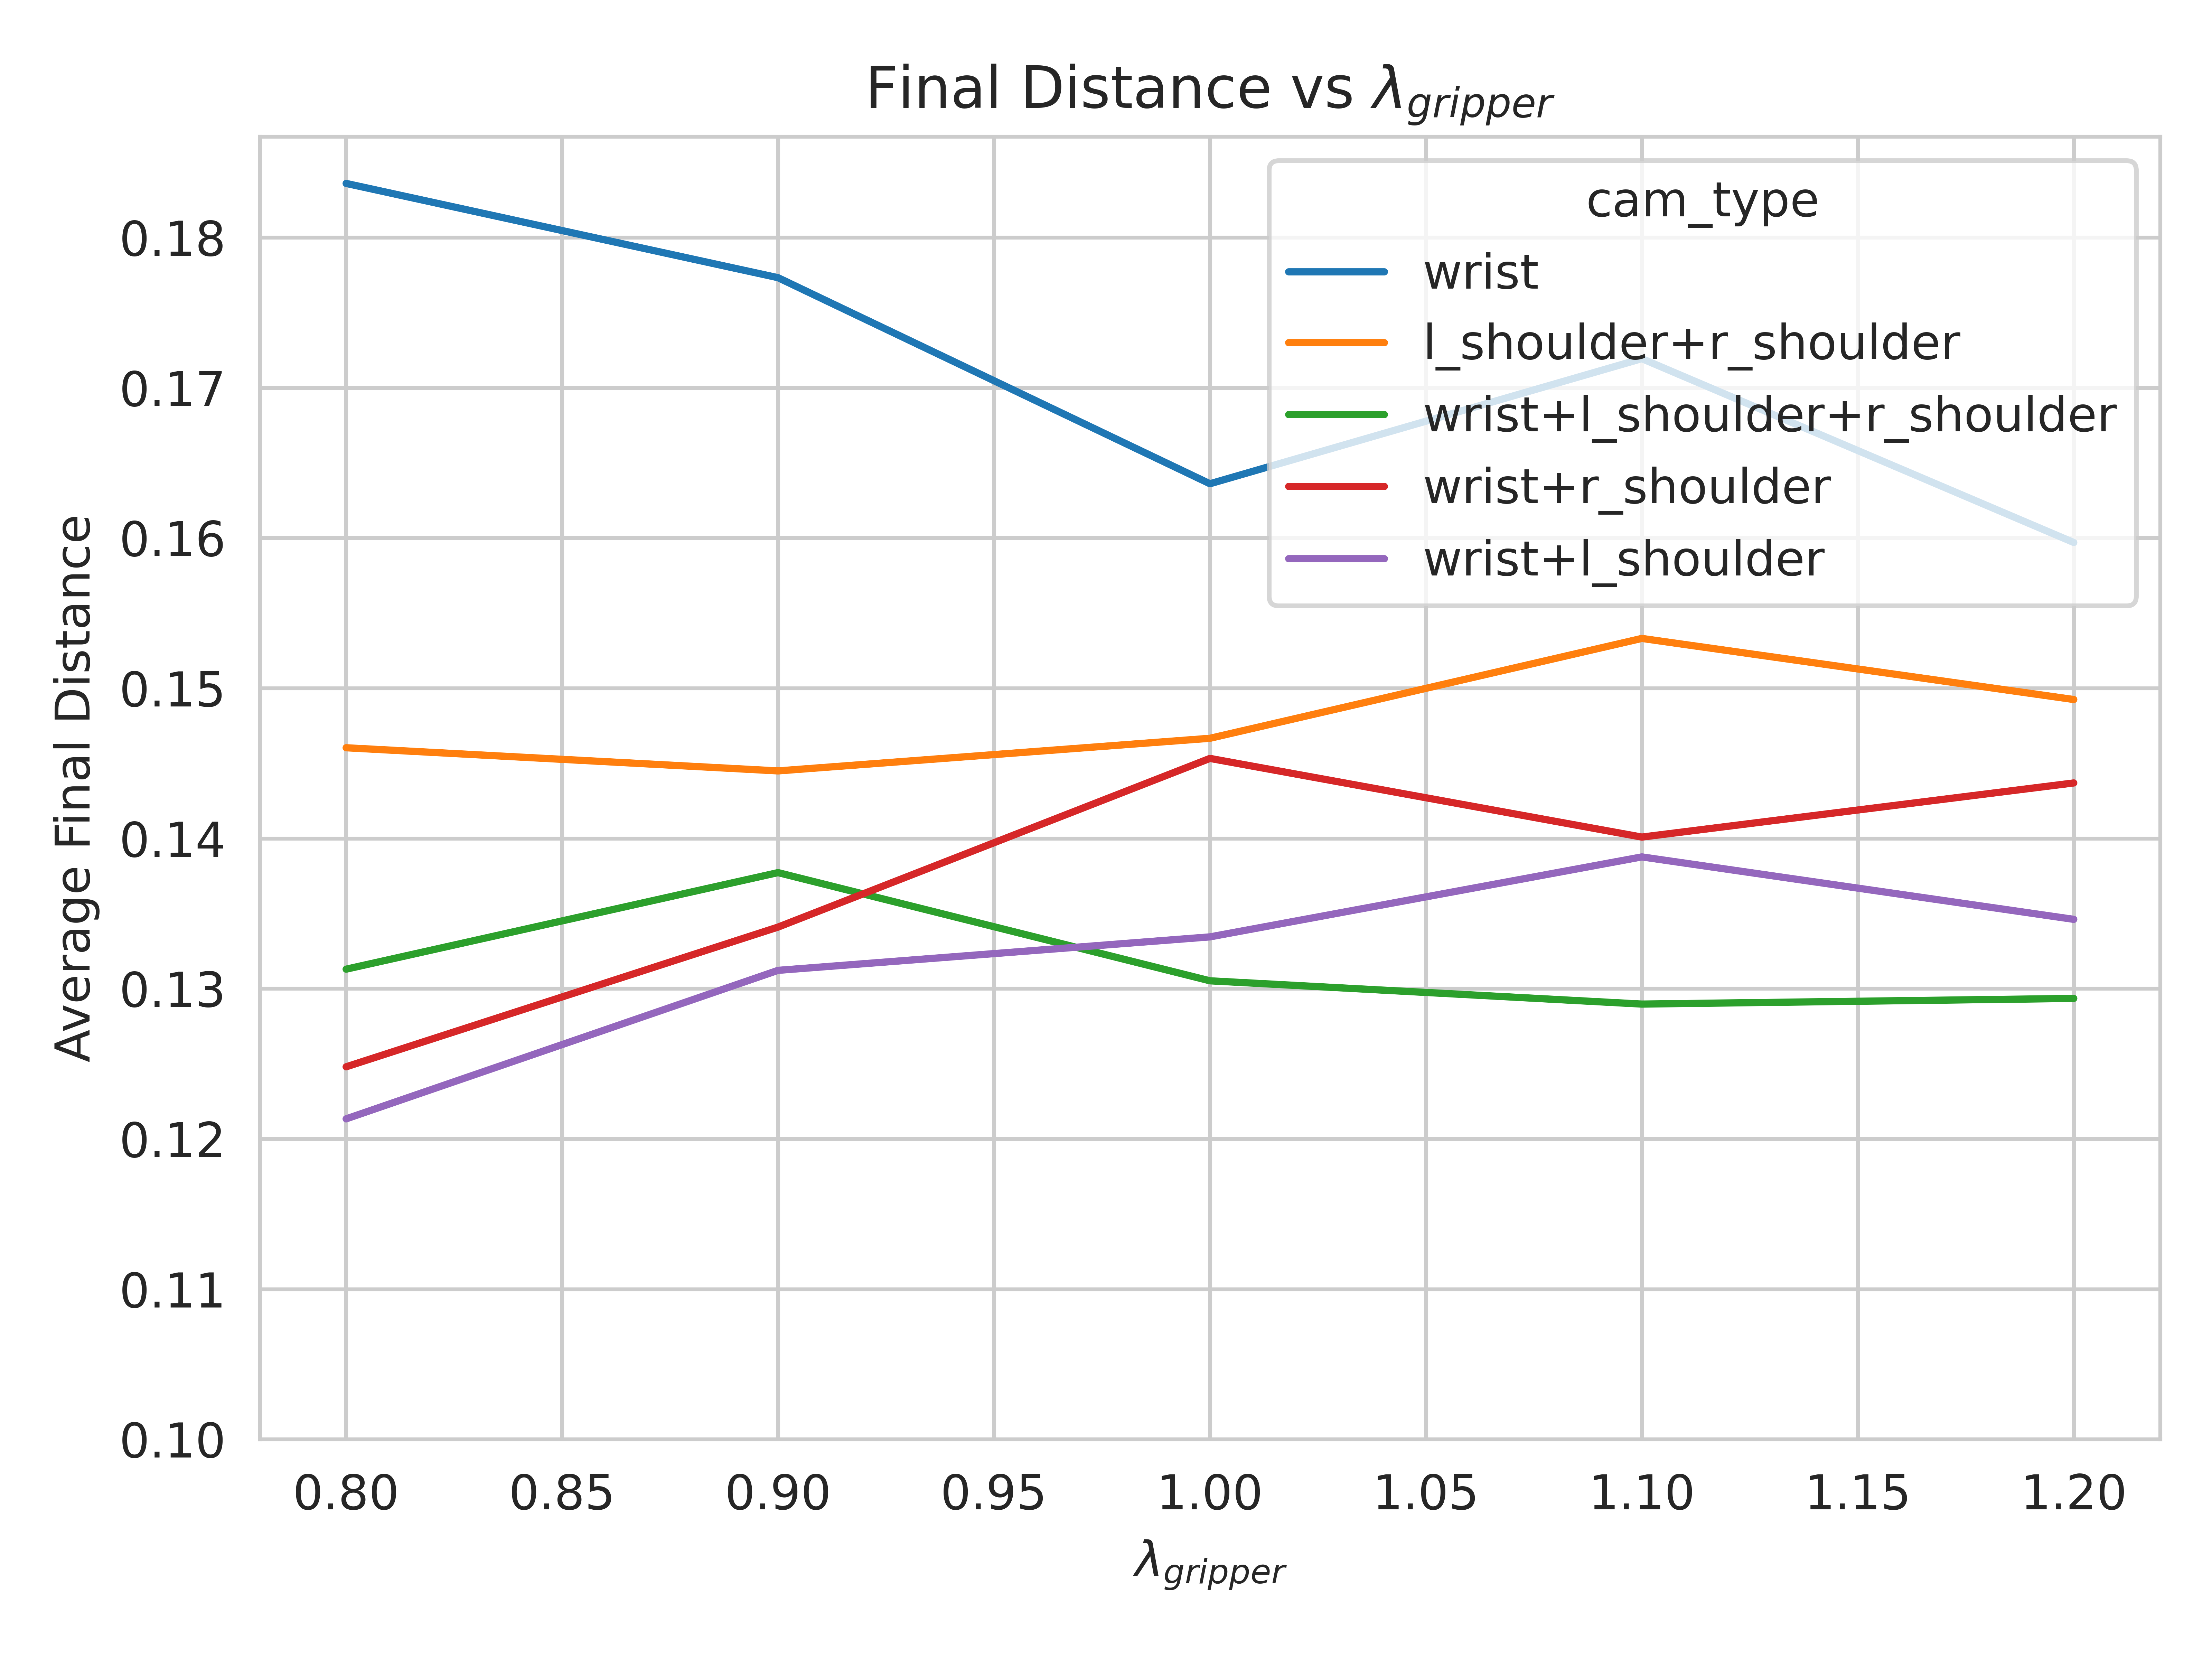
\includegraphics[width=0.7\linewidth]{assets/cam-comb/grasp-simple/tuning-normal-old-policy-lambda-g.png}
    \caption{Average Final Distance vs $\lambda_{gripper}$}\label{subfig:grasp-tuning-lambda-g}
  \end{subfigure}
  \begin{subfigure}{0.45\linewidth}
    \centering
    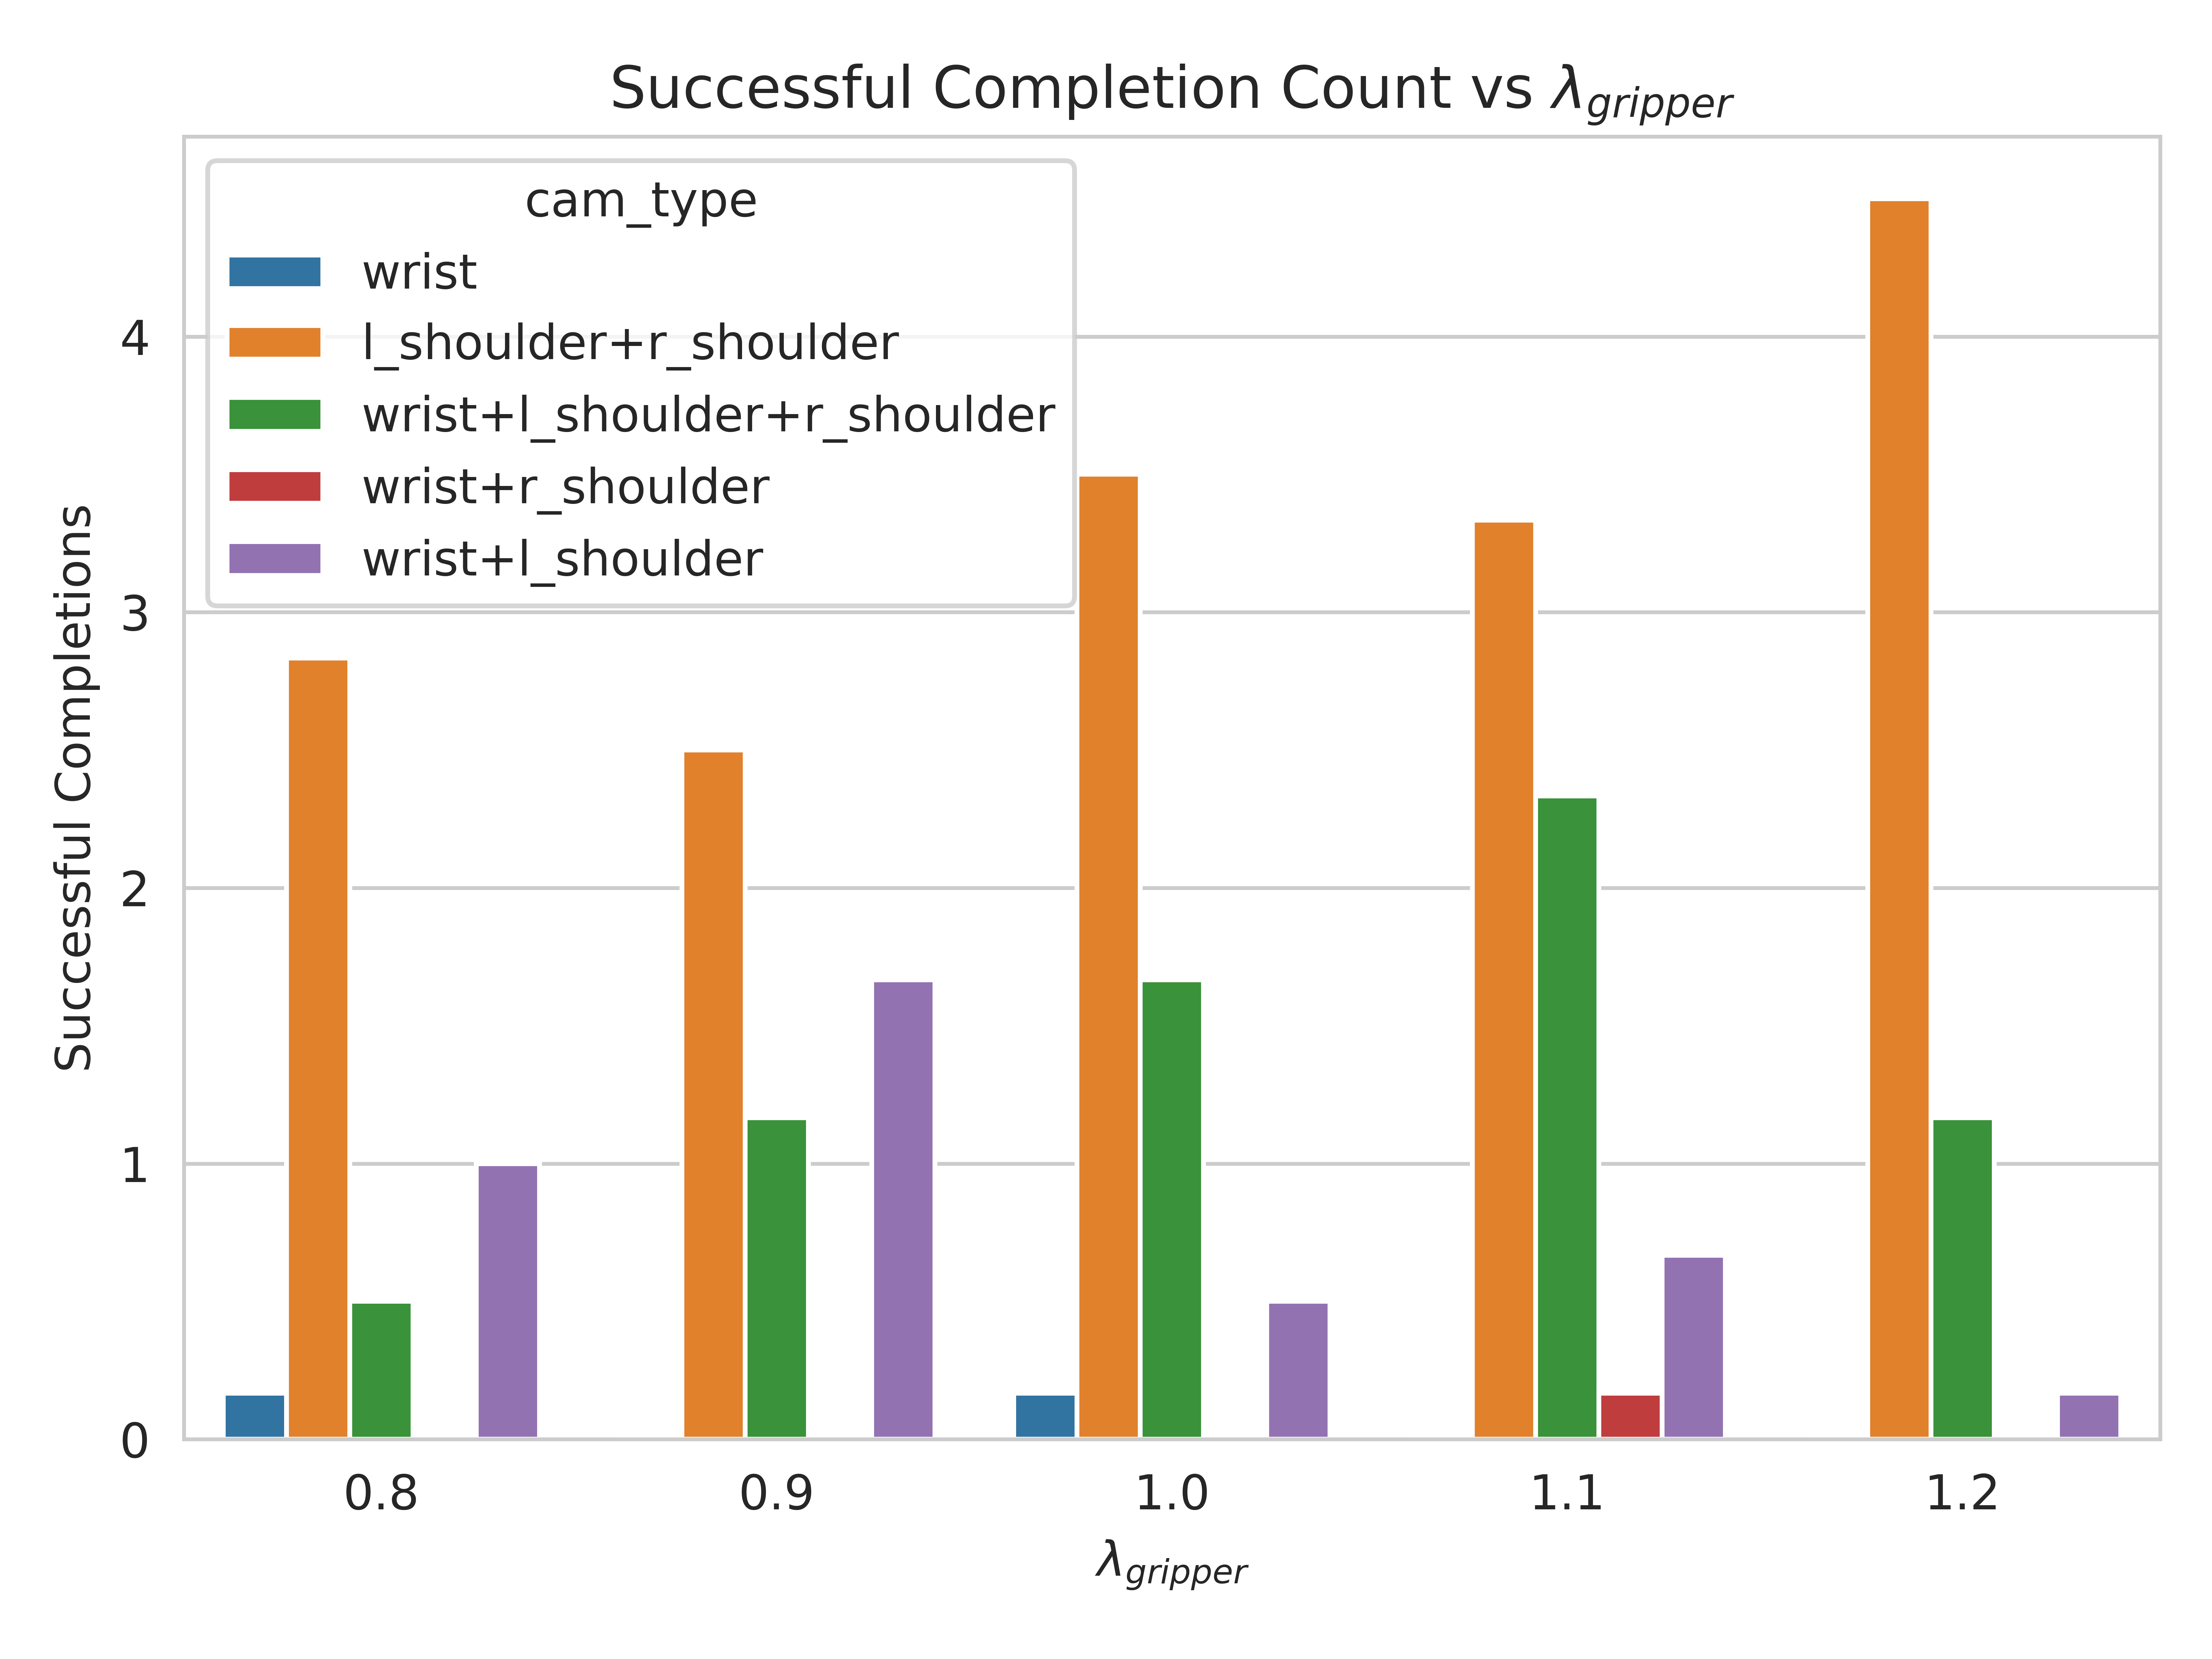
\includegraphics[width=0.7\linewidth]{assets/cam-comb/grasp-simple/tuning-normal-old-policy-success-lambda-g.png}
    \caption{Successful Completions vs $\lambda_{gripper}$}\label{subfig:grasp-tuning-lambda-g-success}
  \end{subfigure}
  \caption{A test run using multiple $\lambda_{gripper}$ values}\label{fig:grasp-tuning-lambda-g}
\end{figure}


\subsubsection{Data Loading Changes}\label{subsec:grasp-data-loading-changes}\todo[color=purple]{the sequential thing, the importnat bit may come later but leave this here for note}
Following the above approach I wanted to streamline the data loading mechanisms that were currently being used. As discussed, (\ref{subsec:reach-data-loading}), the demonstrations are flattened before loading. So, the dataset is of type \verb|[Observation]|. This meant the batch size parameter within the loading directly related to how many frames were getting fed into the system at a time. So, for each epoch we see all the demos, however we only update the parameters of the network per batch and the batch size is determined by the loader.

Realising not training with entirety of a demo in batch. For example if the demonstration has $50$ frames, but the `minibatch\_size' is only $32$ we would see all the demonstrations in dataset given, yet we will see them in slices of $32$. As I omitted shuffling, to preserve the sequential nature of demos the model updates will be done in uncontrolled slices. This is because a demo does not have a fixed episode length and different demos for the same task, can be of different lengths.

So, \verb|DemoDataset| held the data in terms of \verb|list[Demo]|. A drawback is that the demos are different lengths, so more collating and computation needs to be done before feeding this into a torch model. Frames within a demo will be the same sequential order but the demos themselves can be fed in different orders per epoch, which should help with the generalisability of the models trained on th is loader.

\subsection{Masking the Loss}
Next step was to restrain the training to last $k$ steps. Keeping $loss_{bce}$ to be non-zero only while regressing the last few items in the batch. As the batches are now defined as whole demonstrations (see \ref{subsec:grasp-data-loading-changes}), we can make a simple bit mask to match the lengths of demos in our training batch.

Looking at the saved demonstration for this specific task, only the last $14$ frames are labelled `grasp'. The total length of the demo is $64$ observations. To see howw this affects the learning I wanted to test \(\left[15, 28\right]\) which is respectively one more and two times the label length. This made sense as I would compare using all the frames (unbalanced), all the grasp labels and one non-grasp for contrast (unbalanced again but skewing towards grasp) and finally a fully balanced dataset.

I suspected that \(k = 28\) would be the sweet spot, capturing enough closeness data while the labels are balanced. However, Figure \ref{fig:grasp-last-k-final} makes it clear that there this does not really matter in the grand scheme of things. The proficiency of reaching for a single demo is the same. Their success rates also were very similar \todo[color=green]{appendix}, the only difference being $k = 15$ was around 10\% less successful while the other two were within error, hence I did not include it here. This means that the masking does not add any additional benefit to the grasping task, and I will not use it to save on calculations moving forward.

\begin{figure}[htpb]
  \centering
  \includegraphics[width=\linewidth]{assets/cam-comb/grasp-simple/last-k-dist.png}
  \caption{Final Distance Reached with masking}\label{fig:grasp-last-k-final}
\end{figure}\todo{move to appendix if needed}
